\subsection{Conceptos Básicos}
Es uno de los operadores de cruce más utilizados en los MOEAs y es clasificado como centrado en los padres, 
particularmente tiene la propiedad de poder crear cualquier valor en el espacio de búsqueda combinando dos individuos padres.
%
En el SBX en base a dos individuos padres ($p_1$, $p_2$) se generan dos hijos ($c_1$, $c_2$) considerando 
a una distribución de probabilidad.
%
Para tener más control la forma de la distribución de la probabilidad se puede controlar con un índice de distribución 
$\eta_c$ que determina la apertura de la distribución, y por tanto, la capacidad de exploración.
%
Específicamente, un índice de distribución pequeño induce una mayor probabilidad de construir soluciones hijas alejadas de los padres, mientras que con un índice de distribución elevado, la probabilidad de crear soluciones hijas más similares a los padres se incrementa. 
%
El efecto de $\eta_c$ es ilustrado en la Figura \ref{fig:Density_SBX}, donde se muestran las funciones de densidad de dos índices 
de distribución distintos.
%
Específicamente los círculos representan a los padres, y se puede apreciar que con $\eta_c=5$, la probabilidad de crear soluciones 
más cercanas a los padres es mayor que con $\eta_c=2$.
\begin{figure*}[!t]%[H]
\centering
\begin{tabular}{cc}
   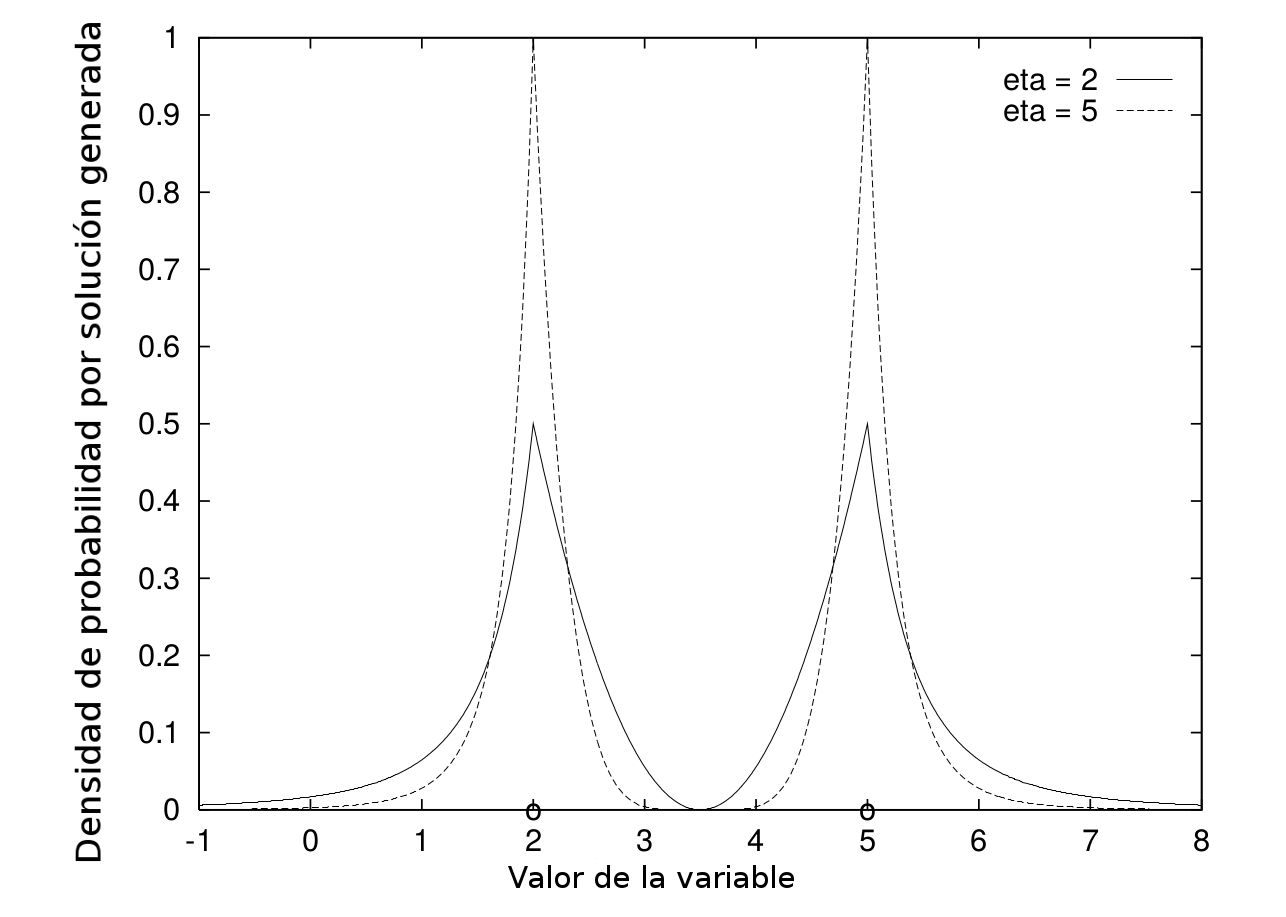
\includegraphics[width=0.5\textwidth]{img/Operadores/DensitySBX.png} &
\end{tabular}
\caption{Función de densidad del operador SBX con índices de distribución 2 y 5.}
\label{fig:Density_SBX}
%\caption{Probability density function SBX with indexes of distribution 1,2 and 5. The red point is a Parent solution.}
\end{figure*}


El SBX tiene la propiedad de preservar una relación entre la media de los valores padres e hijos ($c_1 + c_2 = p_1 + p_2$), 
con lo que se define el factor de dispersión $\beta = | c_1 - c_2| / |p_1 - p_2|$, y en base al valor de $\beta$, podemos
determinar donde quedarían localizados los hijos.
%
En el SBX la probabilidad de distribución para $\beta \in [0, \infty]$ viene dada por:

\begin{equation}
    P(\beta)= 
\begin{cases}
     0.5(\eta_c + 1)\beta^{\eta_c},& \text{si} \quad \beta \leq 1\\
     0.5(\eta_c + 1) \frac{1}{\beta^{\eta_c + 2}} ,& \text{de otra forma}
\end{cases}
\end{equation}

En base a esto, se cumplen las siguientes propiedades:
\begin{itemize}
\item Los valores de las soluciones hijas son equidistantes de los padres.
\item Existe una probabilidad no nula de generar una solución hija en cualquier parte en el espacio independientemente de donde se localicen los padres.
\item La probabilidad de crear un par de soluciones hijas dentro del rango de las soluciones padres es idéntica a la probabilidad de crear dos soluciones hijas fuera de dicho rango.
\end{itemize}

A la hora de implementar esta distribución para dos valores de los individuos padres ($p_1$, $p_2$), se crean los valores  
de los hijos ($c_1$, $c_2$) como combinación lineal de los valores padres con un número aleatorio $u \in [0, 1]$ 
de la forma (\cite{Joel:SBX1994}):
\begin{equation} \label{eq:generar_ind}
\begin{split}
c_1 &= 0.5(1 + \beta(u))p_1 + 0.5(1 - \beta(u)) p_2 \\
c_2 &= 0.5(1 - \beta(u))p_1 + 0.5(1 + \beta(u)) p_2
\end{split}
\end{equation}

Así, para realiza la simulación del parámetro $\beta(u)$, primero se genera un número aleatorio $u \in [0, 1]$, y se utiliza 
en la siguiente fórmula:
\begin{equation} \label{eq:Parametro_beta}
    \beta(u)= 
\begin{cases}
     (2u)^{\frac{1}{\eta_c+1}},& \text{si} \quad u \leq 0.5,\\
     	(\frac{1}{2(1-u)})^{\frac{1}{\eta+1}} ,& \text{de otra forma}
\end{cases}
\end{equation}

Se puede observar que la forma de la distribución no está afectada por los límites de cada variable, en base a este inconveniente, 
los autores \cite{deb1999self} modificaron la ecuación (\ref{eq:Parametro_beta}) de forma que exista una probabilidad cero 
de crear individuos fuera del dominio de la variable, por lo tanto se puede calcular $\beta(u, a)$ en función de un número 
aleatorio $u \in [0,1]$ de la forma:

\begin{equation} \label{eq:sbx_bounds}
    \beta(u, a)= 
\begin{cases}
     (2u(1-\rho_a))^{\frac{1}{\eta_c+1}},& \text{si} \quad u \leq 0.5/(1-\rho_a),\\
     	(\frac{1}{2(1-u(1-\rho_a))})^{\frac{1}{\eta+1}} ,& \text{de otra forma}
\end{cases}
\end{equation}

donde $a=x_i^{(L)}$ es el límite inferior y $b=x_i^{(U)}$ es el límite superior, y $\rho_a = 1/(2 \beta_a^{\eta_c+1})$, donde $\beta_a = 1 +(p_1 - a)/(p_2 - p_1)$.
%
Similarmente, $\rho_b$ es calculado remplazando $\beta_a$ por $\beta_b =  1 + (b - p_2)/(p_2 - p_1)$, así $\beta(u, b)$ es calculado con la ecuación (\ref{eq:sbx_bounds}), generando así dos individuos hijo en base a sus respectivas funciones de distribución $\beta(u,a)$ y $\beta(u,b)$.


En la práctica, se trabajan con funciones de múltiples variables, con lo que hay que generalizar lo anterior.
%
Una forma sencilla sería aplicar lo mismo a cada variable, pero se ha visto que eso es muy disruptivo, con lo que habitualmente
no se cambian todas las variables.
%
Por ejemplo, en la implementación que más se usa en la práctica (jMETAL, NSGA-II, etc.) cuando se aplica el SBX
cada variable sufre el proceso de cruce con una probabilidad igual a 0.5, mientras que en el resto de casos los valores 
se heredaran sin ser alterados (\cite{Joel:NSGAII,Joel:jMetal}).
%
Además, cuando se produce un cruce también aplican intercambios entre las valores generadas 
con probabilidad 0.5, lo que resulta en reflexiones que son analizados posteriormente.
%
Por último, cabe destacar que no se ha podido encontrar variantes del operador SBX en las que en lugar de usar dichas probabilidades
fijas en 0.5, estas sean cambiadas a lo largo de la ejecución.

 \begin{algorithm}[H]
\algsetup{linenosize=\tiny}
\scriptsize
\caption{Operador de Cruce Binario Simulado (SBX)}
\label{alg:SBX_Operator}
\begin{algorithmic}[1]
    \STATE Entrada: Individuos Padre ($P_1, P_2$), Indice de distribución ($\eta_c$), Probabilidad de cruza ($P_c$).
    \STATE Salida: Individuos hijo($C_1, C_2$).
    \STATE $r_1 \leftarrow U[0, 1]$.
    \IF{ $r_1 \leq P_c$}
       \FOR{ cada variable d}
	\IF{ $U[0, 1] \leq 0.5$}
		 \STATE $a = LowBound(d)$.	
		 \STATE $b = UpperBound(d)$.    
		 \STATE $ r_2 \leftarrow U[0, 1]$.
		 \STATE $\beta_a = 1 +(p_1 - a)/(p_2 - p_1)$.
		 \STATE $\rho_a = 1/(2 \beta_a^{\eta_c+1})$.
		 \STATE Utilizar $r_2$ y $\rho_a$ en la ecuación \ref{eq:sbx_bounds} para generar $\beta(u,a)$.  
		 \STATE Generar a $C_1(d)$ utilizando $\beta(u, a)$ en la ecuación \ref{eq:generar_ind}. 
		 \STATE $\beta_b = 1 +(b - p_2)/(p_2 - p_1)$.
		 \STATE $\rho_b = 1/(2 \beta_b^{\eta_c+1})$.
		 \STATE Utilizar $r_2$ y $\rho_b$ en la ecuación \ref{eq:sbx_bounds} para generar $\beta(u,b)$. 
		 \STATE Generar a $C_2(d)$ utilizando $\beta(u, b)$ en la ecuación \ref{eq:generar_ind}.
		 \IF{$ U[0, 1]  \leq 0.5$} 
			 \STATE Intercambiar los valores de $C_1(d)$ con $C_2(d)$. 
		 \ENDIF 
        \ELSE 
	   \STATE $C_1(d) = P_1(d)$. 
	   \STATE $C_2(d) = P_2(d)$.
        \ENDIF 
       \ENDFOR
    \ELSE
	\STATE $C_1 = P_1$
	\STATE $C_2 = P_2$
    \ENDIF
\end{algorithmic}
\end{algorithm}


%
\subsection{Análisis operador de cruce SBX}

La implementación más utilizada del operador SBX se encuentra integrada en el NSGA-II publicada en (\cite{Joel:NSGAII}).
%
Este procedimiento está descrito en el algoritmo \ref{alg:SBX_Operator}, donde destacan dos aspectos clave.
%
El primero está relacionado con la similitud entre los individuos padre y los hijos (líneas 22 y 23).
%
En dicha implementación los valores de las soluciones hijas son heredadas directamente de las soluciones padre con una probabilidad 
fija igual a 0.5, mientras que el resto de las variables son modificadas mediante la distribución de probabilidad propia del SBX.
%
En consecuencia la similitud que existe entre los padres y los hijos depende del número de variables que se consideran en el 
problema de optimización, pues el incremento de la dimensionalidad involucra la creación de soluciones más distantes.

El segundo punto clave, que nunca ha sido analizado en detalle, está relacionado con el conjunto de reflexiones que se 
realizan en las líneas 18 - 20.
%
Después de generar los dos valores que deben ser heredados en los dos hijos, dichos valores son intercambiados entre sí 
con una probabilidad fija del 0.5.
%
En consecuencia, cada vez que las variables son intercambiadas se realiza una reflexión, que puede inducir grandes distancias 
entre los padres y los hijos, a pesar de que el SBX es considerado como un cruce centrado en los padres.
%
La parte izquierda de la Figura~\ref{fig:Simulations_Index_20} ilustra este comportamiento en el operador SBX para dos y tres variables.
%
En esta figura, los padres están identificados con dos puntos rojos, y se ejecutó el operador SBX diez mil veces.
%
Cada uno de los puntos de color negro es una solución hija, con lo que esta figura ilustra las zonas en las que se tienden 
a generar a los hijos.
%
Se puede ver que los valores de cada variable siempre están cercanos a uno de los valores asociados a las variables de los padres. 
%
Sin embargo, debido al proceso de intercambio de valores, las soluciones hijas no siempre se encuentran cercanas a los padres.
%
Particularmente, en el caso de dos dimensiones mostrado, se crean soluciones en la esquina superior izquierda y en la esquina inferior derecha, mientras que los padres están es las esquinas opuestas.
%
A medida que aumenta el número de dimensiones $d$, la probabilidad de que siempre o nunca haya intercambios, y que por tanto, 
la nueva solución esté cercana a uno de los padres es $k^{d} + (1-k)^{d}$, donde $k$ es la probabilidad de realizar un intercambio,
con lo que se produce un decremento exponencial respecto al número de dimensiones.
%
En consecuencia, las reflexiones provocan un alto grado de exploración.
%
En algunos MOPs con alta dimensionalidad en el espacio de las variables, esto podría representar un inconveniente porque las reflexiones localizan soluciones hijas en cada esquina del hipercubo mínimo que contiene a las soluciones padre, lo que significa que el operador original podría inducir un nivel muy bajo de intensificación.

El inconveniente relacionado con las reflexiones puede ser manejado parcialmente implementando restricciones de emparejamiento que traten de cruzar exclusivamente a soluciones similares. 
%
Bajo esta condiciones, el hipercubo sería de menor tamaño, con lo que se induciría un mayor grado de intensificación.
%
Esta puede ser una de las razones por las que el MOEA/D, que incorpora restricciones de apareamiento, ha sido capaz de resolver muchos problemas de forma exitosa.
%
En este trabajo, se trata de resolver esta problemática eliminando el intercambio de variables, 
así como realizando otras modificaciones en el SBX que se describen en la siguiente sección.
%
La ventaja de esta segunda alternativa es que se puede incorporar de forma sencilla en cualquier MOEA.
%

\begin{figure*}
\centering
\begin{tabular}{cc}
   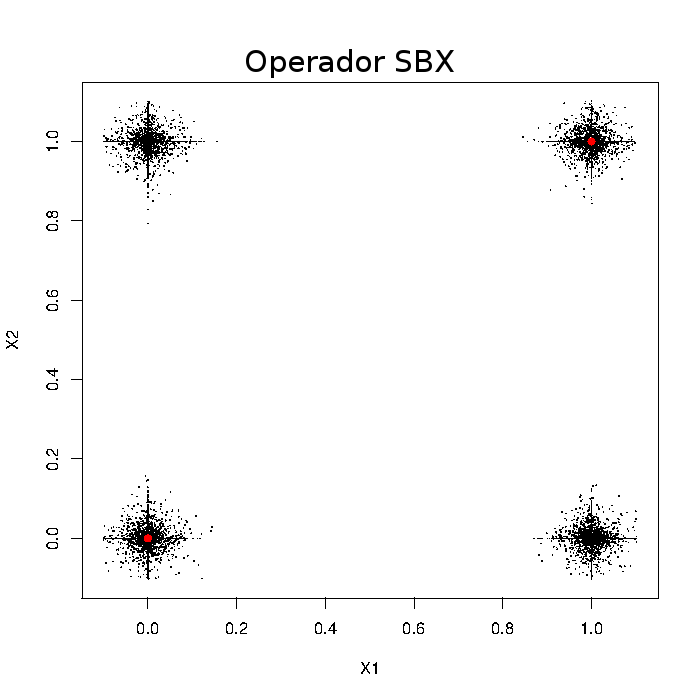
\includegraphics[width=0.3\textwidth]{img/Operadores/SBX_2D_Index_20.png} &
   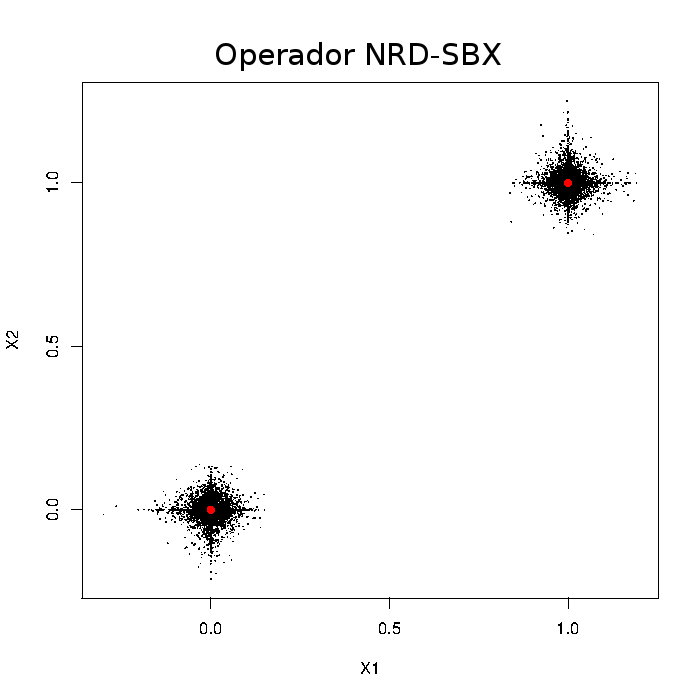
\includegraphics[width=0.3\textwidth]{img/Operadores/DSBX_2D_Index_20.png} \\   
   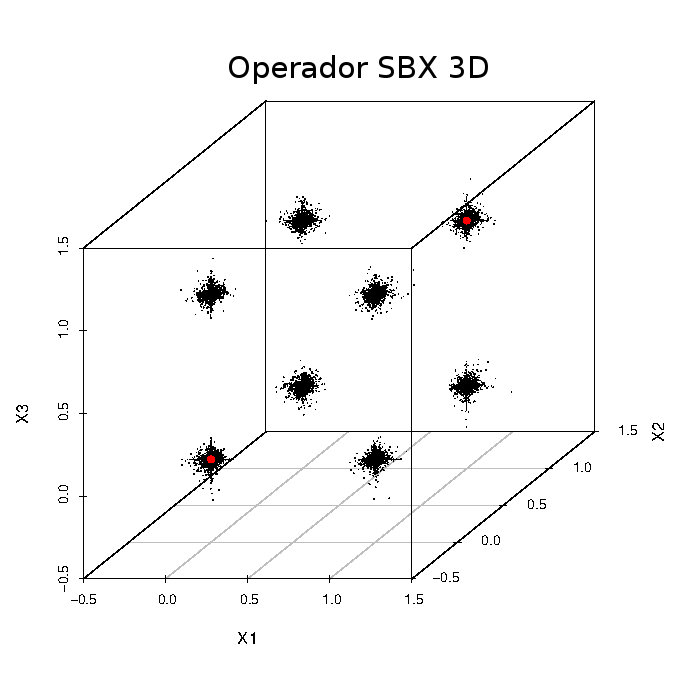
\includegraphics[width=0.3\textwidth]{img/Operadores/SBX_3D_Index_20.png} &
   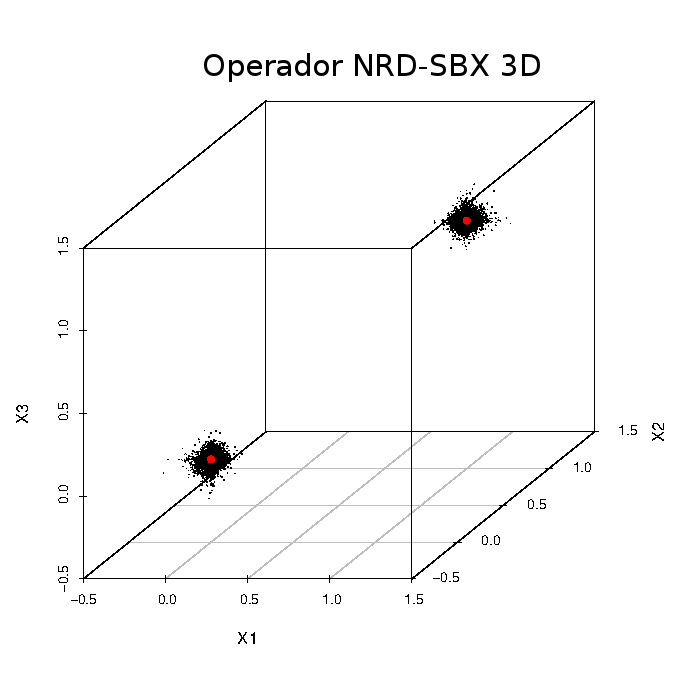
\includegraphics[width=0.3\textwidth]{img/Operadores/DSBX_3D_Index_20.png}  
\end{tabular}
\caption{En la columna izquierda se presenta la simulación del operador  SBX y en la columna de la derecha se presenta el operador NRD-SBX, ambas distribuciones con un índice de distribución de 20.}
%\caption{Simulations SBX left column and NRD-SBX right column with index distribution 20}
\label{fig:Simulations_Index_20}
\end{figure*}


This section is devoted to review some of the most important works that are highly related to the research presented in this paper.
%
First, the most important \MOEAS{} paradigms are defined.
%
Thereafter, some relevant classifications of crossover operators are introduced.
%
Finally, the popular \SBX{} operator, which is used extensively in this paper, is discussed.

\subsection{Multi-objective Evolutionary Algorithms}

In the last years, a large number of \MOEAS{} following different design principles have been devised.
%
In order to better classify them, several taxonomies have been proposed~\cite{Joel:BOOK_MOEAs}.
%
Attending to the principles of design, \MOEAS{} can be based on Pareto dominance, indicators and/or decomposition~\cite{pilat2010evolutionary}.
%
All of them have quite competitive representatives, so in this paper \MOEAS{} belonging to the different groups are taken into account.
%
Particularly, the experimental validation has been carried out by including the Non-Dominated Sorting Genetic Algorithm (NSGA-II)~\cite{Joel:NSGAII}, 
the MOEA based on Decomposition (\MOEAD{})~\cite{Joel:MOEAD}, and the $S$-Metric Selection Evolutionary Multi-objective Optimization Algorithm (\SMSEMOA{})~\cite{Joel:SMSEMOA}.
%
They are representative methods of the domination-based, decomposition-based and indicator-based paradigms, respectively.
%
The following subsections briefly describe each one of these paradigms and introduce the selected methods.

\subsubsection{Domination Based MOEAs - NSGA-II}

One of the most recognized paradigms is the domination based approach.
%
\MOEAS{} belonging to this category are based on the application of the dominance relation to design different components of the EAs, specially the selection phase.
%
Given that the dominance relation does not inherently promotes diversity in the objective space, auxiliary techniques such as niching, crowding and/or clustering 
are usually integrated to obtain an acceptable spread and diversity in the objective space.
%
A critical drawback of methods based on the dominance relation is its scalability in terms of the
dimensionality of the objective space.
%
In fact the selection pressure is substantially reduced as the number of objectives increases.
%
Although some strategies have been developed to deal with this issue \cite{horoba2008benefits} it remains 
as an important drawback for this kind of algorithms.

One of the most popular techniques of this group is the \NSGAII{}.
%
This algorithm \cite{Joel:NSGAII} considers a special selection operator
based on non-dominated sorting and crowding.
%
Non-dominated sorting is used to provide convergence to the Pareto front whereas crowding promotes the preservation of diversity in the objective space.
%
%A recent version is the NSGA-III, which is designed to deal with many-objective problems \cite{Joel:NSGAIII}.%  \cite{horoba2008benefits}.
%

\subsubsection{Decomposition Based MOEAs - MOEA/D}

Decomposition-based \MOEAS{} \cite{Joel:MOEAD} transform a \MOP{} in a set of single-objective optimization problems that are tackled simultaneously.
%
This transformation can be achieved through several approaches.
%
The most popular of them is applying a weighted Tchebycheff function, thus requiring a set of well distributed weights to attain well-spread solutions.
%
An important drawback of this kind of approaches is related to the dependency between the Pareto front geometry and the weights required to attain proper solutions.

\MOEAD{}~\cite{Joel:MOEAD} is a recently designed decomposition-based \MOEA{}.
%
It includes several features such as problem decomposition, weighted aggregation of objectives 
and mating restrictions based on neighborhood definitions.
%
Particularly, the neighborhoods are considered in the mating selection.
%
A popular variant of \MOEAD{} is the \MOEADDE{}, which uses the \DE{} operators~\cite{price2006differential} 
and the polynomial mutation operator~\cite{hamdan2012distribution} in the reproduction phase.
%
Additionally, it has two extra mechanisms for maintaining the population diversity~\cite{zhang2009performance}.
%

\subsubsection{Indicator Based MOEAs - SMS-EMOA}

In multi-objective optimization several quality indicators have been developed to compare the performance of MOEAs.
%
Since these indicators measure the quality of the approximations attained by \MOEAS{}, a paradigm based on the application of these indicators was proposed.
%
Particularly, the indicators replace the Pareto dominance relation with the aim of guiding the optimization process.
%
Among the different indicators, hypervolume is a widely accepted Pareto-compliance quality indicator~\cite{Joel:IGDPlus_And_GDPlus}.
%
One of the main advantages of these algorithms is that indicators usually take into account both the quality and diversity of the solutions,
so no additional mechanisms to preserve diversity are required.
%

A popular and extensively used indicator-based algorithm is the \SMSEMOA{}~\cite{Joel:SMSEMOA}.
%
This algorithm might be considered as hybrid, since it involves both indicators and Pareto dominance concepts.
%
Essentially, it integrates the non-dominated sorting method with the use of the hypervolume metric.
%
Thus, \SMSEMOA{} uses the hypervolume as a density estimator which results in a computationally expensive task.
%
Particularly, the replacement phase erases the individual of the worst ranked front with the minimum contribution to the hypervolume.
%
Taking into account the promising behavior of \SMSEMOA{}, it has been used in our experimental validation.
%

\begin{figure}[!t]
\centering
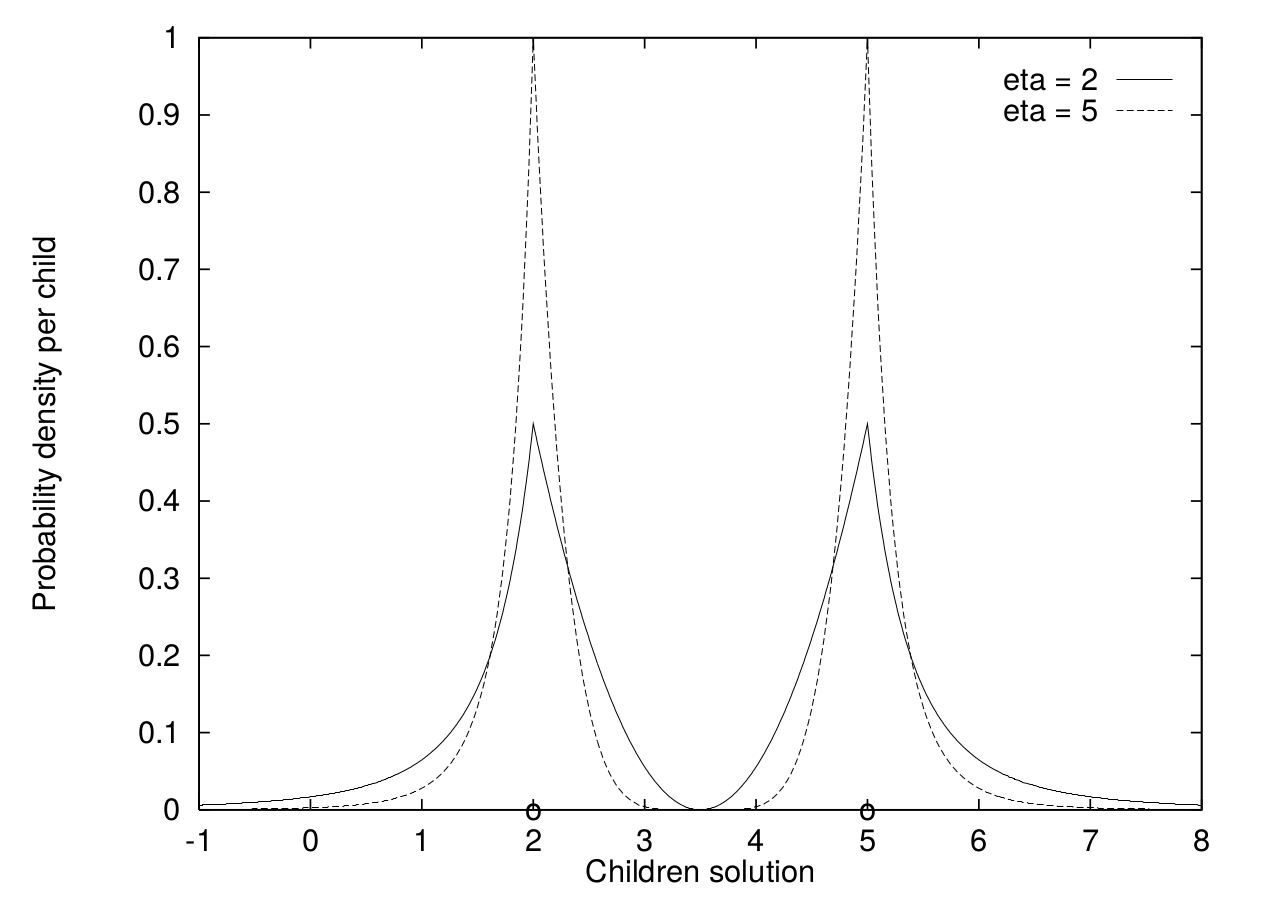
\includegraphics[width=2.5in]{img/Operadores/DensitySBX_English.png}
\caption{Probability density function of the \SBX{} operator with indexes of distribution 2 and 5. The parents are located in 2 and 5 respectively.}
\label{fig:fig_sim}
\end{figure}

\begin{figure}[t]
\centering
\begin{tabular}{cc}
   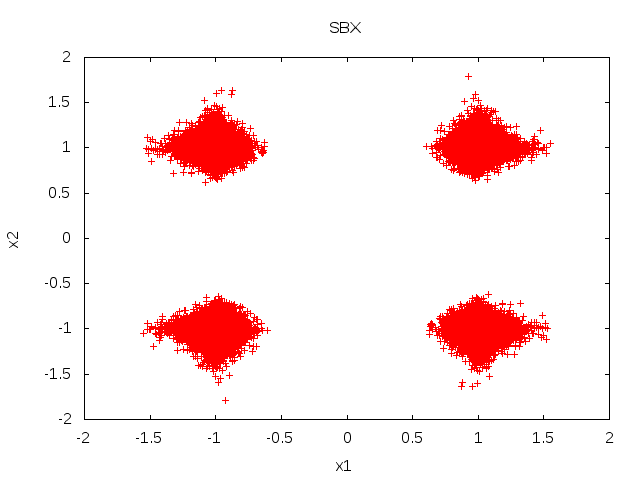
\includegraphics[width=0.23\textwidth]{img/Operadores/SBX_eta_20_2D_pv_1.png} 
   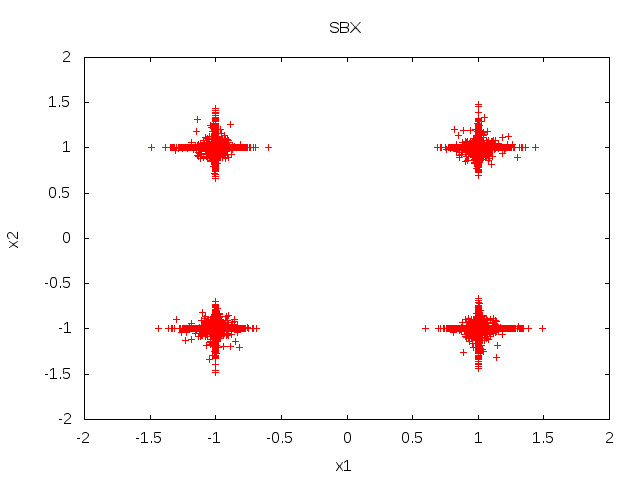
\includegraphics[width=0.23\textwidth]{img/Operadores/SBX_eta_20_2D_pv_01.png} 
\end{tabular}
\caption{Simulations of the \SBX{} operator with a distribution index equal to 20. Parents are located in $P_1=(-1.0, -1.0)$ and $P_2=(1.0, 1.0)$. The left simulation corresponds to a probability of altering a variable ($\delta_1$ in Algorithm \ref{alg:SBX_Operator}) equal to $1.0$ and in the right it corresponds to $0.1$.}
\label{fig:Simulation_pv}
\end{figure}



%
\begin{figure}[t]
\centering
\begin{tabular}{cc}
   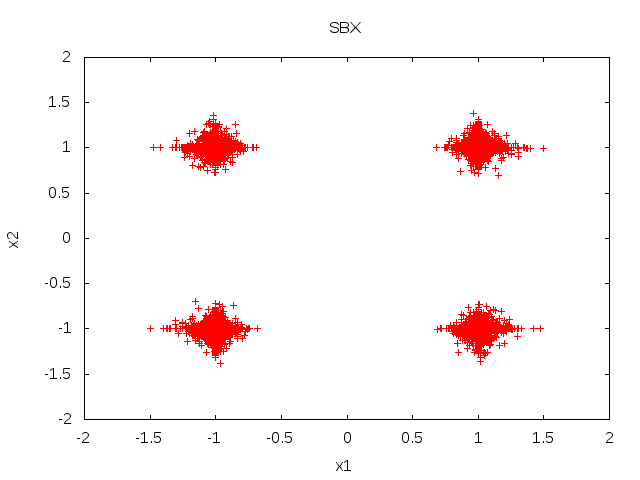
\includegraphics[width=0.23\textwidth]{img/Operadores/SBX_eta_20_2D.png} 
   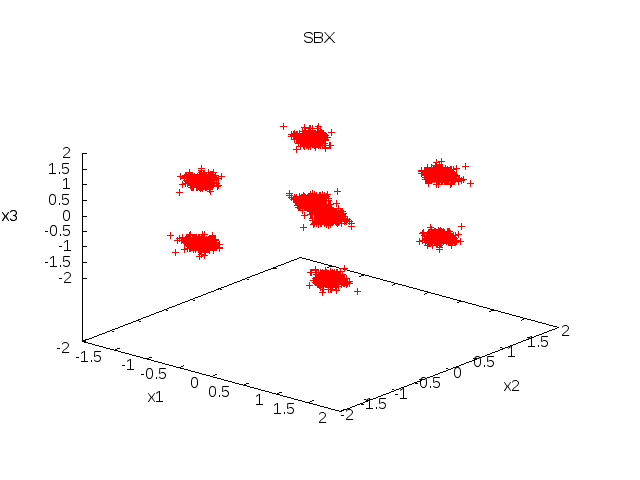
\includegraphics[width=0.23\textwidth]{img/Operadores/SBX_eta_20_3D.png} 
\end{tabular}
\caption{Simulations of the \SBX{} operator with a distribution index equal to 20. Parents are located in $P_1=(-1.0, -1.0)$ and $P_2=(1.0, 1.0)$ and $P_1=(-1.0, -1.0, -1.0)$ and $P_2=(1.0, 1.0, 1.0)$ for two and three variables respectively.}
\label{fig:Simulations_Index_20}
\end{figure}


\subsection{Crossover operators}

The crossover operators are designed to generate offspring solutions using information of the parent solutions.
%
They combine features of two or more parent solutions to generate new candidate solutions.
%
Since several crossover operators have been proposed, some taxonomies have also been provided.
%
The taxonomies are based on features such as the location of new generated solutions or the kinds of relations among the variables.

A popular taxonomy classifies crossover operators into variable-wise operators and vector-wise operators.
%
In the variable wise category, each variable from parent solutions is recombined independently with a certain pre-specified probability to create new values.
%
These operators are specially suitable to deal with separable problems.
%
Some operators belonging to this category are the Blend Crossover (\BLX{})~\cite{eshelman1993real}, and the \SBX{}~\cite{Joel:SBX1994}.
%
Alternatively, the vector-wise recombination operators are designed to take into account the linkage among variables.
%
They usually perform a linear combination of the variable vectors.
%
Some operators belonging to this category are the Unimodal Normally Distributed Crossover (\UNDX{})~\cite{Joel:UNDX}, and the simplex crossover (\SPX{}) \cite{Joel:DE_Storn_SPX}.
%
Additionally, crossover operators can be classified as Parent-Centric and Mean-Centric \cite{jain2011parent}.
%
In Parent-Centric operators, children solutions are created around one of the parent solutions, whereas in Mean-Centric operators, children solutions tend to be created mostly 
around the mean of the participating parent solutions.
%
Among the crossover operators, \SBX{} is probably the most frequently used operator, so this research focuses on this crossover.

\subsubsection{Simulated Binary Crossover - SBX}

The reproduction operators are one of the most relevant components that influence the search process of \EAS{}.
%
Specifically, the crossover and mutation operators are highly related with the diversity of solutions.
%
Hence, the quality of solutions are highly affected by the applied operators.
%
%Particularly, in this paper is discussed the crossover operator.

Simulated Binary Crossover (\SBX{})~\cite{deb1994simulated} is probably the most popular operator for continuous domains and most \MOEAS{} have been extensively
tested with such an operator\cite{Joel:NSGAII,Joel:SMSEMOA}.
%
\SBX{} is classified as Parent-Centric, meaning that two children values ($c_1$ and $c_2$) are created around the parent values ($p_1$ and $p_2$).
%
The process of generating the children values is based on a probability distribution.
%
This distribution controls the spread factor $\beta = |c_1 - c_2 | / |p_1 - p_2|$ defined as the ratio between the spread of the children values and parent values.
%
In order to define this density function a distribution index $\eta_c$ (a user-defined control parameter) alters the exploration capability of the operator.
%
Specifically, a small index induces a larger probability of building children values distant to the parent values, 
whereas high indexes tend to create solutions very similar to the parents as is shown in Figure~\ref{fig:fig_sim}.
%

%Principally, the SBX has non-zero probability of creating any number in the search space by recombining any two parent values from the search space.
%
The probability distribution to create an offspring value is defined as a function of $\beta \in [0, \infty]$ as follows:
%
\begin{equation}
    P(\beta)= 
\begin{cases}
     0.5(\eta_c + 1)\beta^{\eta_c},& \text{if} \quad \beta \leq 1\\
     0.5(\eta_c + 1) \frac{1}{\beta^{\eta_c + 2}} ,& \text{otherwise}
\end{cases}
\end{equation}
%
Based in the mean-preserving property of children values and parent values, \SBX{} has the following properties:
\begin{itemize}
\item Both offspring values are equi-distant from parent values.
\item There exist a non-zero probability to create offspring solutions in the entire feasible space from any two parent values.
\item The overall probability of creating a pair of offspring values within the range of parent values is identical to the overall probability of creating two offspring values outside  
the range of parent values.
\end{itemize}





Therefore, considering two participating parent values ($p_1$ and $p_2$), two offspring values ($c_1$ and $c_2$) can be created as linear combination of parent values with a uniform random number $u \in [0, 1]$, as follows:
\begin{equation} 
\begin{split}
c_1 &= 0.5(1 + \beta(u))p_1 + 0.5(1 - \beta(u)) p_2 \\
c_2 &= 0.5(1 - \beta(u))p_1 + 0.5(1 + \beta(u)) p_2
\end{split}
\end{equation}

The parameter $\beta(u)$ depends on the random number $u$, as follows:
\begin{equation}
    \beta(u)= 
\begin{cases}
     (2u)^{\frac{1}{\eta_c+1}},& \text{if} \quad u \leq 0.5,\\
     	(\frac{1}{2(1-u)})^{\frac{1}{\eta_c +1}} ,& \text{otherwise}
\end{cases}
\end{equation}

The above equation considers an optimization problem with no variable bounds.
%
In most practical problems, each variable is bounded within a lower and upper bound.
%
Thus, the modification of the probability distribution shown in Equation~(\ref{eq:sbx_spread}) 
was proposed~\cite{deb1999self} with the aim of taking into account such bounds.
%
This last variant is extensively used nowadays.

%
\begin{equation} \label{eq:sbx_spread}
    \beta(u)= 
\begin{cases}
     (2u(1-\gamma))^{\frac{1}{\eta_c+1}},& \text{if} \quad u \leq 0.5/(1-\gamma),\\
     	(\frac{1}{2(1-u(1-\gamma))})^{\frac{1}{\eta_c +1}} ,& \text{otherwise}
\end{cases}
\end{equation}
\begin{equation} \label{eq:child_1}
c_1 = 0.5(1 + \beta(u))p_1 + 0.5(1-\beta(u))p_2
\end{equation}
\begin{equation} \label{eq:child_2}
c_2 = 0.5(1 + \beta(u))p_1 + 0.5(1-\beta(u))p_2
\end{equation}

In this case, the child $c_1$ which is nearest to $p_1$ is calculated according to the Equation (\ref{eq:child_1}).
%
Considering that $p_1 < p_2$ and with a lower bound equal to $a$, $\gamma = 1/(\alpha^{\eta_c + 1})$, where $\alpha = 1 + (p_1 - a) / (p_2 - p_1)$.
%
Similarly, the second child $c_2$ is computed with $\alpha = 1 + (b-p_2)/(p_2 - p_1)$, where $b$ correspond to the upper bound.
%
Then, the second child is computed as is indicated in Equation (\ref{eq:child_2}).

\begin{algorithm}[t]
\algsetup{linenosize=\tiny}
\scriptsize
\caption{Simulated Binary Crossover (\SBX{})}
\label{alg:SBX_Operator}
\begin{algorithmic}[1]
    \STATE Input: Parents ($P_{1}, P_{2}$), Distribution index ($\eta_c$), Crossover probability ($P_c$).
    \STATE Output: Children ($C_{1}, C_{2}$).
    \IF{ $U[0, 1] \leq P_c$}
       \FOR{ each variable d}
	\IF{ $U[0, 1] \leq  \delta_1$} \label{alg:inherit_variable}
		\STATE Generate $C_{1,d}$ with Equations (\ref{eq:sbx_spread}) and (\ref{eq:child_1}).
		\STATE Generate $C_{2,d}$ with Equations (\ref{eq:sbx_spread}) and (\ref{eq:child_2}).
		 \IF{$ U[0, 1]  \leq  (1 - \delta_2) $} 
			\STATE Swap $C_{1,d}$ with $C_{2,d}$.
		 \ENDIF
        \ELSE
	   \STATE $C_{1,d} = P_{1, d}$.
	   \STATE $C_{2,d} = P_{2, d}$.
        \ENDIF
       \ENDFOR
    \ELSE
	\STATE $C_{1} = P_{1}$.
	\STATE $C_{2} = P_{2}$.
    \ENDIF
\end{algorithmic}
\end{algorithm}

Note that as reported in~\cite{Joel:SBX1994} several extensions of the \SBX{} to problems with multiple
variables might be provided.
%
Authors considered a simple strategy for choosing the variables to cross~\cite{Joel:UNDX}.
%
Specifically, each variable is crossed with probability 0.5, following the principles of uniform crossover.
%
Authors recognized the important implications on the linkage among variables of such decisions.
%
In any case, this is the most typical way of applying \SBX{} in problems with multiple variables nowadays.
%

\subsubsection{Implementation and analyses of SBX operator}

This section discusses some of the main characteristics of the most currently used implementation of the \SBX{} operator for problems with multiple variables.
%
Essentially, three key components that might affect its performance are discussed.
%
Firstly, as already mentioned it alters each variable with a fixed probability equal to $0.5$.
%
If this probability value is increased, the children tend to be more distant to the parents, since in average 
more variables are modified simultaneously.
%
In separable problems, altering only one variable might be adequate.
%
However, for non-separable problems altering several variables simultaneously seems more promising.
%
The implications of varying this probability is illustrated in Figure~\ref{fig:Simulation_pv}, where a problem
with two variables is taken into account.
%
In the right side a low probability is used and it provokes a bias to explore by keeping some values intact
creating a figure similar to a cross in the two-dimensional case.
%
This feature might be suitable for separable problems.
%
Alternatively, the left side shows that when using a high probability this bias disappears, which could be 
more suitable for non-separable problems.
%
Note that this probability is somewhat related with the distribution index in the sense that both have a
direct effect on the similarity between parents and children.
%
%Otherwise, a low probability value is suitable for objective functions that are separable \cite{ma2016multiobjective}, due that few decision variables are modified by the crossover operation.
%
\begin{figure}[t]
\centering
\begin{tabular}{c}
   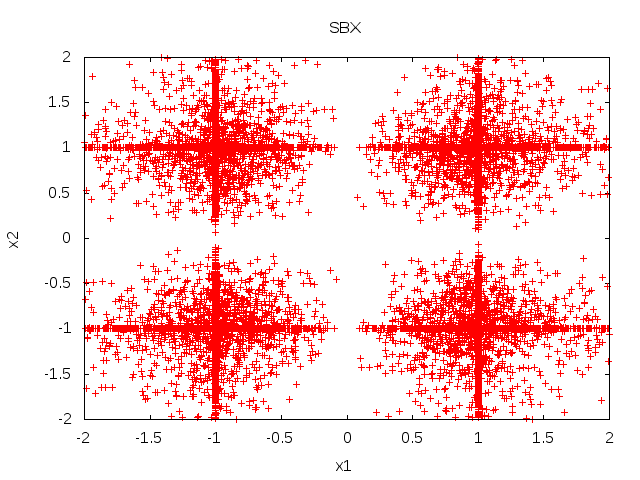
\includegraphics[width=0.24\textwidth]{img/Operadores/SBX_eta_2.png}  %&
   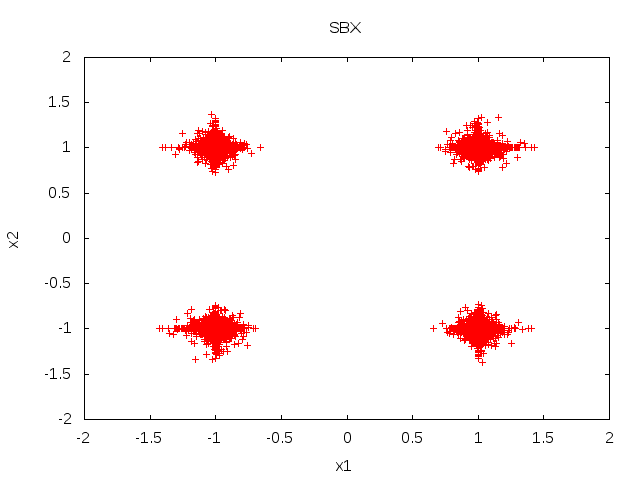
\includegraphics[width=0.24\textwidth]{img/Operadores/SBX_eta_20.png} 
\end{tabular}
\caption{Simulation of the \SBX{} operator sampling $10,000$ children values, the parents are located in $P_1=(-1.0, -1.0)$ and $P_2=(1.0, 1.0)$. The left and right are with a distribution index of $2$ and $20$ respectively.}
\label{fig:Simulation_Case_3}
\end{figure}

The second key issue is that after generating the two child values with the \SBX{} distribution, such values
are interchanged with a fixed probability that is usually set to $0.5$, i.e. the value closer to parent $p_1$ is
not always inherited by $c_1$.
%
This is a feature that is not usually discussed but it is important for the obtained performance.
%
In some contexts this probability is known as ``Variable uniform crossover probability'' 
\cite{tuvsar2007differential} or ``Discrete Recombination'' \cite{muhlenbein1993predictive}.
%
Since in multi-objective optimization more diversity is maintained these swaps might produce a high disruptive operator.
%
In fact, in some sense due to this action it is not so clear that \SBX{} can be categorized as a parent-centric operator.
%
These interchanges between the children has the effect of performing multiple ``reflections'' in the search space.
%
When increasing the dimensions of the decision variables the number of regions covered increases exponentially 
as is illustrated in Figure \ref{fig:Simulations_Index_20} where cases with two and three decision variables are taken into account.
%
Note also that this feature has a considerable effect on the distance between parents and offspring.

Finally, the last component is the distribution index, which is probably the most well known feature of the \SBX{}.
%
A low index results in greater exploration levels.
%
In fact, a distribution index equal to one has a similar effect to the Fuzzy Recombination Operator \cite{voigt1995fuzzy}.
%
The effect of applying different indexes is illustrated in Figure~\ref{fig:Simulation_Case_3} where the left side
considers a low index value whereas the right side takes into account a higher index value, which creates 
new candidate solutions that are more similar to the parents.
%

The \SBX{} implementation is shown in Algorithm \ref{alg:SBX_Operator}.
%
This pseudocode is based on the implementation that is integrated in the NSGA-II code published by Deb et al. \cite{Joel:NSGAII} and which
is the most popular variant nowadays.
%
As an input it requires two parents ($P_1$ and $P_2$) and it creates two children ($C_1$ and $C_2$).
%
The first and second key components commented previously correspond to the lines 5 and 8, respectively. 
%
As is usual, for the basic case, \SBX{} is configured with $\delta_1 = \delta_2 = 0.5$ and $\eta_c = 20$.
%
It is important take into account that this implementation does not consider the dimension of the decision variables 
or the stopping criteria to set any of its internal parameters.

\subsection{Propuesta}

Based on the previous analyses and with the aim of inducing an appropriate balance between 
exploration and intensification, the following modifications are proposed.
%
First, the probability to modify a variable ($\delta_1$) is dynamically
modified during the execution.
%
The rationality behind this modification is to increase the exploration capability in the initial stages
by altering simultaneously several variables and then, as the evolution proceeds reduce the number of variables
that are modified.
%
The value of $\delta_1$ is changed in base of a linear decreasing model, where initially it is fixed to $1.0$ and 
then it is decreased so that at the half of total generations is equal to $0.5$.
%
This last value is maintained until the end of the execution, i.e. from the half of the execution it behaves as the 
traditional \SBX{} implementation.
%
Equation (\ref{eqn:linear}) is the one used to set the value of $\delta_1$, where $G_{Elapsed}$ is the current generation 
and $G_{End}$ is the total number of generations.

In a similar way, the second change is related to the probability of performing reflections ($1 - \delta_2$).
%
In this case $\delta_2$ is also updated as in Equation (\ref{eqn:linear}), meaning that the probability of performing
a reflection increases from $0.0$ to $0.5$ during the execution.
%
This modification is performed with the aim of avoiding the disruptive behavior of interchanging the variables at the
first generations because this might result in very drastic modifications.
%
Once that the individuals converge to certain degree it might make more sense to perform such reflections.
%
Thus, this probability is increased to $0.5$ which is the value used in the standard implementation of \SBX{}.

\begin{equation}\label{eqn:linear}
	\delta_1 = \delta_2 = max \left (0.5, 1.0 - \frac{G_{Elapsed}}{G_{End}} \right )
\end{equation}

Finally, the distribution index is also changed during the execution. 
%
At the first stages a low distribution index is induced with the aim of increasing the exploration capabilities 
of \SBX{}.
%
Then, it is linearly incremented which has the effect of closing the distribution curve, meaning that more intensification is
promoted.
%
The linear increment is governed by Equation (\ref{eqn:index_eta}), meaning that the distribution index is altered
from $2$ to $22$.
%
Note that modifications similar to this last one have been explored previously 
\cite{zitzler1999multiobjective}, \cite{hamdan2012distribution}.
%

\begin{equation}\label{eqn:index_eta}
 \eta_c = 2 + 20 \times \left ( \frac{G_{Elapsed}}{G_{End}} \right)
\end{equation}

\subsection{Resultados}

\begin{table}[t]
\centering
\scriptsize
\caption{References points for the HV indicator}
\label{tab:ReferencePoints}
\begin{tabular}{cc}
\hline
\textbf{Instances} & \textbf{Reference Point} \\ \hline
WFG1-WFG9 & $[2.1, ...,2m+0.1]$ \\
DTLZ 1, 2, 4 & $[1.1, ..., 1.1]$ \\
DTLZ 3, 5, 6 & $[3, ..., 3]$ \\
DTLZ7 & $[1.1, ..., 1.1, 2m]$ \\
UF 1-10 & $[2, ..., 2]$ \\ \hline
\end{tabular}
\end{table}


% Please add the following required packages to your document preamble:
% \usepackage{multirow}
% \usepackage{graphicx}
\begin{table*}[t]
\centering

\caption{Statistical Information of Metrics with two objectives}
\label{tab:Metrics_2}
\resizebox{\textwidth}{!}{%
\begin{tabular}{|c|c|c|c|c|c|c|c|c|c|c|c|c|c|c|c|c|c|c|}
\hline
\multirow{2}{*}{} & \multicolumn{6}{c|}{NSGA-II} & \multicolumn{6}{c|}{MOEA/D} & \multicolumn{6}{c|}{SMS-EMOA} \\ \cline{2-19} 
 & 1 & 2 & 3 & 4 & 5 & DE & 1 & 2 & 3 & 4 & 5 & DE & 1 & 2 & 3 & 4 & 5 & DE \\ \hline
Average HV & 0.88 & 0.90 & 0.90 & 0.91 & 0.93 & \textbf{0.94} & 0.87 & 0.87 & 0.87 & 0.90 & \textbf{0.91} & \textbf{0.91} & 0.88 & 0.89 & 0.87 & 0.91 & 0.92 & \textbf{0.93} \\ \hline
%Best Counts HV & 2 & 1 & 0 & 1 & 8 & \textbf{11} & 2 & 0 & 2 & 2 & 8 & \textbf{9} & 0 & 1 & 1 & 5 & 6 & \textbf{10} \\ \hline
%\multicolumn{1}{|l|}{Average Best Difference HV} & \multicolumn{1}{l|}{0.068} & \multicolumn{1}{l|}{0.057} & \multicolumn{1}{l|}{0.053} & \multicolumn{1}{l|}{0.039} & \multicolumn{1}{l|}{0.019} & \multicolumn{1}{l|}{\textbf{0.017}} & \multicolumn{1}{l|}{0.053} & \multicolumn{1}{l|}{0.048} & \multicolumn{1}{l|}{0.049} & \multicolumn{1}{l|}{0.024} & \multicolumn{1}{l|}{\textbf{0.013}} & \multicolumn{1}{l|}{0.014} & \multicolumn{1}{l|}{0.074} & \multicolumn{1}{l|}{0.064} & \multicolumn{1}{l|}{0.081} & \multicolumn{1}{l|}{0.045} & \multicolumn{1}{l|}{0.028} & \multicolumn{1}{l|}{\textbf{0.019}} \\ \hline
Average IGD+ & 0.12 & 0.09 & 0.11 & 0.07 & 0.06 & \textbf{0.05} & 0.14 & 0.12 & 0.14 & 0.09 & 0.08 & \textbf{0.07} & 0.13 & 0.11 & 0.14 & 0.08 & 0.07 & \textbf{0.05} \\ \hline
%Best Counts IGD+ & 2 & 1 & 1 & 1 & 8 & \textbf{10} & 3 & 0 & 2 & 3 & 6 & \textbf{9} & 0 & 2 & 0 & 3 & \textbf{9} & \textbf{9} \\ \hline
%\multicolumn{1}{|l|}{Average Best Difference IGD+} & \multicolumn{1}{l|}{0.086} & \multicolumn{1}{l|}{0.052} & \multicolumn{1}{l|}{0.077} & \multicolumn{1}{l|}{0.035} & \multicolumn{1}{l|}{0.021} & \multicolumn{1}{l|}{\textbf{0.016}} & \multicolumn{1}{l|}{0.075} & \multicolumn{1}{l|}{0.059} & \multicolumn{1}{l|}{0.072} & \multicolumn{1}{l|}{0.025} & \multicolumn{1}{l|}{0.019} & \multicolumn{1}{l|}{\textbf{0.008}} & \multicolumn{1}{l|}{0.093} & \multicolumn{1}{l|}{0.071} & \multicolumn{1}{l|}{0.101} & \multicolumn{1}{l|}{0.038} & \multicolumn{1}{l|}{0.030} & \multicolumn{1}{l|}{\textbf{0.017}} \\ \hline
\end{tabular}%
}
\end{table*}

% Please add the following required packages to your document preamble:
% \usepackage{multirow}
% \usepackage{graphicx}
\begin{table*}[t]
\centering
\caption{Statistical Information of Metrics with three objectives}
\label{tab:Metrics_3}
\resizebox{\textwidth}{!}{%
\begin{tabular}{|c|c|c|c|c|c|c|c|c|c|c|c|c|c|c|c|c|c|c|}
\hline
\multirow{2}{*}{} & \multicolumn{6}{c|}{NSGA-II} & \multicolumn{6}{c|}{MOEA/D} & \multicolumn{6}{c|}{SMS-EMOA} \\ \cline{2-19} 
 & 1 & 2 & 3 & 4 & 5 & DE & 1 & 2 & 3 & 4 & 5 & DE & 1 & 2 & 3 & 4 & 5 & DE \\ \hline
Average HV & \textbf{0.87} & 0.84 & \textbf{0.87} & \textbf{0.87} & \textbf{0.87} & 0.85 & 0.84 & 0.84 & 0.84 & \textbf{0.86} & \textbf{0.86} & 0.85 & 0.90 & 0.89 & 0.88 & \textbf{0.91} & \textbf{0.91} & \textbf{0.91} \\ \hline
%Best Counts HV & 1 & 2 & 1 & 4 & 4 & \textbf{7} & 1 & 2 & 1 & 2 & 5 & \textbf{8} & 3 & 2 & 0 & 2 & 5 & \textbf{7} \\ \hline
%\multicolumn{1}{|l|}{Average Best Difference HV} & \multicolumn{1}{l|}{0.019} & \multicolumn{1}{l|}{0.047} & \multicolumn{1}{l|}{0.020} & \multicolumn{1}{l|}{\textbf{0.014}} & \multicolumn{1}{l|}{\textbf{0.014}} & \multicolumn{1}{l|}{0.032} & \multicolumn{1}{l|}{0.036} & \multicolumn{1}{l|}{0.041} & \multicolumn{1}{l|}{0.038} & \multicolumn{1}{l|}{0.016} & \multicolumn{1}{l|}{\textbf{0.013}} & \multicolumn{1}{l|}{0.027} & \multicolumn{1}{l|}{0.038} & \multicolumn{1}{l|}{0.038} & \multicolumn{1}{l|}{0.049} & \multicolumn{1}{l|}{\textbf{0.019}} & \multicolumn{1}{l|}{0.027} & \multicolumn{1}{l|}{\textbf{0.019}} \\ \hline
Average IGD+ & 0.13 & 0.16 & 0.13 & \textbf{0.12} & \textbf{0.12} & 0.13 & 0.15 & 0.14 & 0.15 & \textbf{0.11} & \textbf{0.11} & 0.13 & 0.11 & 0.11 & 0.13 & \textbf{0.09} & \textbf{0.09} & 0.13 \\ \hline
%Best Counts IGD+ & 0 & 2 & 2 & 4 & 3 & \textbf{8} & 2 & 2 & 0 & 2 & 4 & \textbf{9} & 1 & 3 & 0 & 3 & 5 & \textbf{7} \\ \hline
%\multicolumn{1}{|l|}{Average Best Difference IGD+} & \multicolumn{1}{l|}{0.029} & \multicolumn{1}{l|}{0.061} & \multicolumn{1}{l|}{0.027} & \multicolumn{1}{l|}{0.023} & \multicolumn{1}{l|}{\textbf{0.020}} & \multicolumn{1}{l|}{0.032} & \multicolumn{1}{l|}{0.053} & \multicolumn{1}{l|}{0.048} & \multicolumn{1}{l|}{0.053} & \multicolumn{1}{l|}{\textbf{0.015}} & \multicolumn{1}{l|}{\textbf{0.015}} & \multicolumn{1}{l|}{0.030} & \multicolumn{1}{l|}{0.047} & \multicolumn{1}{l|}{0.040} & \multicolumn{1}{l|}{0.062} & \multicolumn{1}{l|}{\textbf{0.020}} & \multicolumn{1}{l|}{0.024} & \multicolumn{1}{l|}{0.069} \\ \hline
\end{tabular}%
}
\end{table*}
\begin{table*}[t]
\centering
\caption{Summary of Statistical Tests}
\label{tab:statistical_Tests}
\begin{tabular}{|c|c|c|c|c|c|c|c|c|c|c|c|c|c|c|c|}
\hline
\multicolumn{16}{|c|}{NSGA-II} \\ \hline
 & \multicolumn{3}{c|}{1} & \multicolumn{3}{c|}{2} & \multicolumn{3}{c|}{3} & \multicolumn{3}{c|}{4} & \multicolumn{3}{c|}{5} \\ \hline
 & $\uparrow$ & $\downarrow$ & $\longleftrightarrow$ & $\uparrow$ & $\downarrow$ & $\longleftrightarrow$ & $\uparrow$ & $\downarrow$ & $\longleftrightarrow$ & $\uparrow$ & $\downarrow$ & $\longleftrightarrow$ & $\uparrow$ & $\downarrow$ & $\longleftrightarrow$ \\ \hline
\textbf{HV-2obj} & 16 & 29 & 47 & 6 & 61 & 25 & 28 & 19 & 45 & 31 & 23 & 38 & \textbf{54} & 3 & 35 \\ \hline
\textbf{HV-3obj} & 15 & 19 & 42 & 12 & 50 & 14 & 17 & 15 & 44 & \textbf{33} & 10 & 33 & 26 & 9 & 41 \\ \hline
\textbf{IGD-2obj} & 14 & 30 & 48 & 4 & 60 & 28 & 25 & 17 & 50 & 33 & 19 & 40 & \textbf{52} & 2 & 38 \\ \hline
\textbf{IGD-3obj} & 14 & 18 & 44 & 13 & 44 & 19 & 18 & 15 & 43 & \textbf{33} & 15 & 28 & 23 & 9 & 44 \\ \hline
% \end{tabular}
% \end{table*}

% \begin{table*}[]
% \centering
% \caption{My caption}
% \label{my-label}
% \begin{tabular}{|c|c|c|c|c|c|c|c|c|c|c|c|c|c|c|c|}
\hline
\hline
\multicolumn{16}{|c|}{MOEA/D} \\ \hline
 & \multicolumn{3}{c|}{1} & \multicolumn{3}{c|}{2} & \multicolumn{3}{c|}{3} & \multicolumn{3}{c|}{4} & \multicolumn{3}{c|}{5} \\ \hline
 & $\uparrow$ & $\downarrow$ & $\longleftrightarrow$ & $\uparrow$ & $\downarrow$ & $\longleftrightarrow$ & $\uparrow$ & $\downarrow$ & $\longleftrightarrow$ & $\uparrow$ & $\downarrow$ & $\longleftrightarrow$ & $\uparrow$ & $\downarrow$ & $\longleftrightarrow$ \\ \hline
\textbf{HV-2obj} & 15 & 33 & 44 & 10 & 60 & 22 & 25 & 26 & 41 & 39 & 18 & 35 & \textbf{57} & 9 & 26 \\ \hline
\textbf{HV-3obj} & 10 & 22 & 44 & 12 & 39 & 25 & 11 & 19 & 46 & 24 & 10 & 42 & \textbf{38} & 5 & 33 \\ \hline
\textbf{IGD-2obj} & 16 & 31 & 45 & 9 & 60 & 23 & 23 & 27 & 42 & 37 & 17 & 38 & \textbf{57} & 7 & 28 \\ \hline
\textbf{IGD-3obj} & 12 & 22 & 42 & 13 & 43 & 20 & 13 & 24 & 39 & 30 & 9 & 37 & \textbf{40} & 10 & 26 \\ \hline
% \end{tabular}
% \end{table*}

% \begin{table*}[]
% \centering
% \caption{My caption}
% \label{my-label}
% \begin{tabular}{|c|c|c|c|c|c|c|c|c|c|c|c|c|c|c|c|}
\hline
\hline
\multicolumn{16}{|c|}{SMS-EMOA} \\ \hline
 & \multicolumn{3}{c|}{1} & \multicolumn{3}{c|}{2} & \multicolumn{3}{c|}{3} & \multicolumn{3}{c|}{4} & \multicolumn{3}{c|}{5} \\ \hline
 & $\uparrow$ & $\downarrow$ & $\longleftrightarrow$ & $\uparrow$ & $\downarrow$ & $\longleftrightarrow$ & $\uparrow$ & $\downarrow$ & $\longleftrightarrow$ & $\uparrow$ & $\downarrow$ & $\longleftrightarrow$ & $\uparrow$ & $\downarrow$ & $\longleftrightarrow$ \\ \hline
\textbf{HV-2obj} & 9 & 35 & 48 & 7 & 43 & 42 & 16 & 31 & 45 & 41 & 9 & 42 & \textbf{53} & 8 & 31 \\ \hline
\textbf{HV-3obj} & 7 & 21 & 48 & 9 & 35 & 32 & 13 & 21 & 42 & 27 & 6 & 43 & \textbf{31} & 4 & 41 \\ \hline
\textbf{IGD-2obj} & 10 & 34 & 48 & 15 & 48 & 29 & 12 & 33 & 47 & 41 & 12 & 39 & \textbf{55} & 6 & 31 \\ \hline
\textbf{IGD-3obj} & 8 & 20 & 48 & 13 & 30 & 33 & 9 & 19 & 48 & 22 & 5 & 49 & \textbf{27} & 5 & 44 \\ \hline
\end{tabular}
\end{table*}


This section is devoted to analyze the results obtained with the dynamic variants of \SBX{} (\DSBX{}).
%
The novel crossover operator was integrated with \NSGAII{}, \MOEAD{} and \SMSEMOA{}.
%
First, three variants that alter only one of each of the components previously discussed are analyzed.
%
Then, a case that alters two of them simultaneously is taken into account.
%
The WFG \cite{Joel:WFG}, DTLZ \cite{Joel:DTLZ_2} and UF \cite{zhang2009performance} test problems have been used for our purpose.
%
Our experimental validation also includes the variant of Differential Evolution known as DEMO~\cite{tuvsar2007differential}
with the aim of comparing our extension of \SBX{} with other well-known operators.

Given that all the methods are stochastic algorithms, each execution was repeated $35$ times with different seeds.
%
The common configuration in all of them was the following: the stopping criterion was set to $25,000$ generations, 
the population size was fixed to 100, WFG test problems were configured with two and three objectives, and 24 variables
were considered, where 20 of them are distance parameters and 4 of them are position parameters.
%
In the case of the DTLZ test instances, the number of decision variables were set to $n=M+r-1$, where $r=\{5, 10, 20\}$ 
for DTLZ1, DTLZ2 to DTLZ6 and DTLZ7 respectively, as is suggested in\cite{Joel:DTLZ_2}.  
% 
In the UF benchmark set the number of decision variables were set to 10.
%
Finally, the polynomial mutation was used with a mutation probability equal to $1/n$ and with a distribution index equal to 50, 
whereas for the cases that used the \SBX{}, the crossover probability was set to $0.9$ and the distribution index
was set to 20.
%
The additional parameterization of each algorithm was as follows:
\begin{itemize}
\item \textbf{DEMO}: CR = 0.3 and F = 0.5.
\item \textbf{SMS-EMOA}: offset = 100.
\item \textbf{MOEA/D}: size of neighborhood = 10, max updates by sub-problem (nr) = 2 and $\delta = 0.9$.
\end{itemize}

In order to compare the fronts obtained by the different methods the 
normalized hypervolume (HV) and IGD+ was taken into account.
%
The reference points used for the hypervolume indicator are shown in the Table \ref{tab:ReferencePoints} 
and are similar to the ones used in \cite{Joel:Kuhn_Munkres, Joel:OperatorAHX}.

In order to statistically compare the results (IGD+ and HV values), the following statistical tests were performed. 
%
First a Shapiro-Wilk test was performed to check whatever or not the values of the results followed a Gaussian distribution. 
%
If, so, the Levene test was used to check for the homogeneity of the variances. 
%
If samples had equal variance, an ANOVA test was done; if not, a Welch test was performed. 
%
For non-Gaussian distributions, the nonparametric Kruskal-Wallis test was used to test whether samples are drawn 
from the same distribution. 
%
An algorithm $X$ is said to win algorithm $Y$ when the differences between them are statistically significant, and
the mean and median obtained by $X$ are higher (in HV) or lower (in IGD+) than the mean and median achieved by $Y$.


\subsection{Analysis of isolated components}

In this section we discuss about the independent effect of each component that is dynamically modified.
%
%Particularly, the jMetalcpp framework \cite{Joel:jMetal}  was used to perform our executions.
%
%Taking into account the stochastic behavior of MOEAs, $35$ independent executions were run.
%
%In all of them, the stopping criteria was set to $25,000$ generations and the size of the population was fixed to $100$.
%
The effect of each component is analyzed through four cases, based in the Algorithm \ref{alg:SBX_Operator}.
%
Each case is described as follows:

\begin{itemize}
\item \textbf{Case 1}: The standard SBX operator where $\delta_1 = \delta_2 = 0.5$ and $\eta_c = 20$.
\item \textbf{Case 2}: The value $\delta_1$ is updated according to Equation~(\ref{eqn:linear}),  $\delta_2=0.5$ and $\eta_c = 20$.
\item \textbf{Case 3}: The value $\delta_2$ is updated according to Equation~(\ref{eqn:linear}), $\delta_1=0.5$ and $\eta_c = 20$.
\item \textbf{Case 4}: The distribution index is updated according to Equation~(\ref{eqn:index_eta}), $\delta_1=\delta_2=0.5$.
\end{itemize}


In order to analyze the performance of each Case (Case 5 is discussed later), Tables \ref{tab:Metrics_2} and
\ref{tab:Metrics_3} shows information about the Normalized Hyper-volume 
(HV)~\cite{zitzler1999multiobjective} and about the Inverted Generational Distance Plus (IGD+)~\cite{Joel:IGDPlus_And_GDPlus}.
%
Specifically, the mean of the HV and IGD+ for all considered problems are shown for two and three objectives.
%
It is clear that case 4 outperforms case 1, case 2 and case 3 both with two and three objectives in all the tested algorithms.
%
Therefore, increasing the distribution index during the execution seems to be the most beneficial action.
%
This occurs because the initially open distribution curve leads to a higher degree of exploration, whereas as the evolution
proceeds more intensification is promoted.
%
On the other hand, case 2 presented a lower performance than case 1 when taking into account three objectives.
%
Thus, it seems that altering almost all the variables convert the new approach into a too disruptive operator.
%
Perhaps, altering $\delta_1$ in a different way might provide better results, but this is left as a future work.

Previous analyses are only based on the mean obtained for all the problems.
%
However, depending on the problem the performance might vary.
%
This is analyzed in the following section.
%
Additionally, more detailed results are available\footnote{https:\//\//github.com\//joelchaconcastillo\//SBX\_CEC2018.}.


\subsection{Simultaneous modification of several components}

Based on the previously discussed results, a variant of the \SBX{} is proposed where the case 3 and case 4 are mixed, 
i.e. both $\delta_2$ and the distribution index are updated dynamically.
%
Since case 2 did not report significant benefits, the updating mechanism for $\delta_1$ was discarded.
%
Specifically in our case 5, Algorithm \ref{alg:SBX_Operator} is configured as follows.
%
The parameter $\delta_1$ is fixed to $0.5$, i.e. in a similar way than the standard \SBX{}.
%
Following the case 3, $\delta_2$ is updated according to Equation~(\ref{eqn:linear}).
%
Finally, according to case 4 $\eta_c$ is updated in base of Equation~(\ref{eqn:index_eta}).

Attending to the mean HV and IGD+ obtained by the case 5 (see Tables~\ref{tab:Metrics_2} and \ref{tab:Metrics_3})
it is clear that integrating case 3 and case 4 is beneficial.
%
The advantages are clearer in the case of two objectives, whereas in the case of three objectives, case 4
and case 5 are similar in terms of mean performance.
%
Moreover, results attained with case 5 are superior to the ones obtained with \DE{} in three objectives, whereas
when using the traditional \SBX{} results deteriorate.
%
Thus, when properly configuring a \DSBX{} results similar or superior to DEMO could be obtained.

Finally, since previous analyses only consider the mean among all the benchmark problems, an additional analyses
was developed to better understand the contributions of the different cases.
%
Particularly, pair-wise statistical tests among all the five cases that consider \SBX{} and \DSBX{} were carried out.
%
This was performed independently for \NSGAII{}, \MOEAD{} and \SMSEMOA{}.
%
Results of these statistical tests are shown in Table~\ref{tab:statistical_Tests}.
%
For each algorithm and case, the column ``$\uparrow$'' reports the number of comparisons where the statistical tests 
confirmed the superiority of the corresponding case, whereas the column ``$\downarrow$'' reports the number of cases 
where it was inferior and ``$\longleftrightarrow$'' indicates the number of comparisons where 
differences were not statistically significant.
%%
The advantages of case 5 are quite clear.
%
Only in the case of \NSGAII{} with three objectives, case 4 could outperform the results obtained by case 5.
%
Thus, by properly combining several dynamic modification, results can be improved further.
%
Moreover, results confirm the advantages of our proposals when compared to the standard \SBX{} (case 1).
%
The only case that is not clearly superior to the standard \SBX{} is the case number 2, as it was previously discussed.
%

%This might occurs for the ranking mechanism of this MOEA.
%
%Since that the NSGA-II applies a binary tournament selection based in dominance concept and crowding procedure, thus an appropriate level of diversity is maintained.
%
%As result some promising regions are reached.

%
%Although that with three objective the Case 4 and our proposal have similar average results.
%
%The average difference with the best indicates that our proposal is mostly closest to the best values.
%
%This since that it shows $0.020$ in the ``Average Best Difference'' IGD+ against the Case 4 with $0.023$.
%
%Also, inspecting the statistical tests, the Case 4 has more loses than our proposal ($10$ against $9$ and $15$ against $9$) of the HV and IGD+ respectively.
%
%However, the MOEA/D and SMS-EMOA which are more elitist algorithms and do not consider the dominance concept at all, are not affected in this sense.
%
%Anyway, our proposal and the Case 3 reports significantly better results that the normal SBX (Case 1), in fact this could evidence that variate the distribution index among the execution has an important effect.




%In the Table \ref{tab:statistical_Tests} is showed a summary of the statistical tests, where are considered the HV and IGD+ both in two and three objectives.
%
%Based in the statistical tests (Table \ref{tab:statistical_Tests}), the Case 4 which correspond to the dynamic distribution index, yield better results than Case 1, Case 2 and Case 3.
%
%
%In the second place is the Case 3, it increases the probability of interchange a variable based in a linear model, this might occurs since that at the first stages are avoided disruptive modifications.
%
%Therefore, the promising regions are not adequately explored, although that this case does not yield the best results, it still outperforms the standard SBX (Case 1).
%
%Also can be noticed that the results of the HV are similar that with the IGD+.
%





%Although that the DE variants provides better average results than our proposal considering two objective, our proposal provides near solutions to the best, showing its stability.
%
%Also according the number of objectives increase to three our proposal provides the best results.
%
%The main reason is that DE is seriously deteriorated as the number of objectives increases, also it converges in a fast way, since it incorporates an aggressive selection operator.
%

%Despite the fact that DE variants have high ``Best Count'' values, in average it is improved by the Case 4 and Case 5, this might occurs because DE is directly influenced by the probability crossover ($CR$) and the mutation factor ($F$), therefore in some instances the DE variants attained the best results, and in other instances the solutions are far from the Pareto front.
%

%On the other hand, our proposal shows a robust behavior in the state-of-the-art MOEAs, in fact the ``Average Best Difference'' is low both with two objectives and three objectives that confirms the stability and superiority of our proposal.
%
% % Please add the following required packages to your document preamble:
% % \usepackage{multirow}
% % \usepackage{graphicx}
% \begin{table*}[]
% \centering
% \caption{Statistical Information of Metrics}
% \label{my-label}
% \resizebox{\textwidth}{!}{%
% \begin{tabular}{|l|c|c|c|c|c|c|c|c|c|c|c|c|c|c|c|c|c|c|c|}
% \hline
% \multicolumn{2}{|l|}{\multirow{2}{*}{}} & \multicolumn{6}{c|}{NSGA-II} & \multicolumn{6}{c|}{MOEA/D} & \multicolumn{6}{c|}{SMS-EMOA} \\ \cline{3-20} 
% \multicolumn{2}{|l|}{} & 1 & 2 & 3 & 4 & 5 & 6 & 1 & 2 & 3 & 4 & 5 & 6 & 1 & 2 & 3 & 4 & 5 & 6 \\ \hline
% \multirow{6}{*}{2 Objectives} & Average HV & 0.88 & 0.90 & 0.90 & 0.91 & 0.93 & \textbf{0.94} & 0.87 & 0.87 & 0.87 & 0.90 & \textbf{0.91} & \textbf{0.91} & 0.88 & 0.89 & 0.87 & 0.91 & 0.92 & \textbf{0.93} \\ \cline{2-20} 
%  & Best Counts HV & 2 & 1 & 0 & 1 & 8 & \textbf{11} & 2 & 0 & 2 & 2 & 8 & \textbf{9} & 0 & 1 & 1 & 5 & 6 & \textbf{10} \\ \cline{2-20} 
%  & \multicolumn{1}{l|}{Average Best Difference HV} & \multicolumn{1}{l|}{0.068} & \multicolumn{1}{l|}{0.057} & \multicolumn{1}{l|}{0.053} & \multicolumn{1}{l|}{0.039} & \multicolumn{1}{l|}{0.019} & \multicolumn{1}{l|}{\textbf{0.017}} & \multicolumn{1}{l|}{0.053} & \multicolumn{1}{l|}{0.048} & \multicolumn{1}{l|}{0.049} & \multicolumn{1}{l|}{0.024} & \multicolumn{1}{l|}{\textbf{0.013}} & \multicolumn{1}{l|}{0.014} & \multicolumn{1}{l|}{0.074} & \multicolumn{1}{l|}{0.064} & \multicolumn{1}{l|}{0.081} & \multicolumn{1}{l|}{0.045} & \multicolumn{1}{l|}{0.028} & \multicolumn{1}{l|}{\textbf{0.019}} \\ \cline{2-20} 
%  & Average IGD+ & 0.12 & 0.09 & 0.11 & 0.07 & 0.06 & \textbf{0.05} & 0.14 & 0.12 & 0.14 & 0.09 & 0.08 & \textbf{0.07} & 0.13 & 0.11 & 0.14 & 0.08 & 0.07 & \textbf{0.05} \\ \cline{2-20} 
%  & Best Counts IGD+ & 2 & 1 & 1 & 1 & 8 & \textbf{10} & 3 & 0 & 2 & 3 & 6 & \textbf{9} & 0 & 2 & 0 & 3 & \textbf{9} & \textbf{9} \\ \cline{2-20} 
%  & \multicolumn{1}{l|}{Average Best Difference IGD+} & \multicolumn{1}{l|}{0.086} & \multicolumn{1}{l|}{0.052} & \multicolumn{1}{l|}{0.077} & \multicolumn{1}{l|}{0.035} & \multicolumn{1}{l|}{0.021} & \multicolumn{1}{l|}{\textbf{0.016}} & \multicolumn{1}{l|}{0.075} & \multicolumn{1}{l|}{0.059} & \multicolumn{1}{l|}{0.072} & \multicolumn{1}{l|}{0.025} & \multicolumn{1}{l|}{0.019} & \multicolumn{1}{l|}{\textbf{0.008}} & \multicolumn{1}{l|}{0.093} & \multicolumn{1}{l|}{0.071} & \multicolumn{1}{l|}{0.101} & \multicolumn{1}{l|}{0.038} & \multicolumn{1}{l|}{0.030} & \multicolumn{1}{l|}{\textbf{0.017}} \\ \hline
% \multirow{6}{*}{3 Objectives} & Average HV & \textbf{0.87} & 0.84 & \textbf{0.87} & \textbf{0.87} & \textbf{0.87} & 0.85 & 0.84 & 0.84 & 0.84 & \textbf{0.86} & \textbf{0.86} & 0.85 & 0.90 & 0.89 & 0.88 & \textbf{0.91} & \textbf{0.91} & \textbf{0.91} \\ \cline{2-20} 
%  & Best Counts HV & 1 & 2 & 1 & 4 & 4 & \textbf{7} & 1 & 2 & 1 & 2 & 5 & \textbf{8} & 3 & 2 & 0 & 2 & 5 & \textbf{7} \\ \cline{2-20} 
%  & \multicolumn{1}{l|}{Average Best Difference HV} & \multicolumn{1}{l|}{0.019} & \multicolumn{1}{l|}{0.047} & \multicolumn{1}{l|}{0.020} & \multicolumn{1}{l|}{\textbf{0.014}} & \multicolumn{1}{l|}{\textbf{0.014}} & \multicolumn{1}{l|}{0.032} & \multicolumn{1}{l|}{0.036} & \multicolumn{1}{l|}{0.041} & \multicolumn{1}{l|}{0.038} & \multicolumn{1}{l|}{0.016} & \multicolumn{1}{l|}{\textbf{0.013}} & \multicolumn{1}{l|}{0.027} & \multicolumn{1}{l|}{0.038} & \multicolumn{1}{l|}{0.038} & \multicolumn{1}{l|}{0.049} & \multicolumn{1}{l|}{\textbf{0.019}} & \multicolumn{1}{l|}{0.027} & \multicolumn{1}{l|}{\textbf{0.019}} \\ \cline{2-20} 
%  & Average IGD+ & 0.13 & 0.16 & 0.13 & \textbf{0.12} & \textbf{0.12} & 0.13 & 0.15 & 0.14 & 0.15 & \textbf{0.11} & \textbf{0.11} & 0.13 & 0.11 & 0.11 & 0.13 & \textbf{0.09} & \textbf{0.09} & 0.13 \\ \cline{2-20} 
%  & Best Counts IGD+ & 0 & 2 & 2 & 4 & 3 & \textbf{8} & 2 & 2 & 0 & 2 & 4 & \textbf{9} & 1 & 3 & 0 & 3 & 5 & \textbf{7} \\ \cline{2-20} 
%  & \multicolumn{1}{l|}{Average Best Difference IGD+} & \multicolumn{1}{l|}{0.029} & \multicolumn{1}{l|}{0.061} & \multicolumn{1}{l|}{0.027} & \multicolumn{1}{l|}{0.023} & \multicolumn{1}{l|}{\textbf{0.020}} & \multicolumn{1}{l|}{0.032} & \multicolumn{1}{l|}{0.053} & \multicolumn{1}{l|}{0.048} & \multicolumn{1}{l|}{0.053} & \multicolumn{1}{l|}{\textbf{0.015}} & \multicolumn{1}{l|}{\textbf{0.015}} & \multicolumn{1}{l|}{0.030} & \multicolumn{1}{l|}{0.047} & \multicolumn{1}{l|}{0.040} & \multicolumn{1}{l|}{0.062} & \multicolumn{1}{l|}{\textbf{0.020}} & \multicolumn{1}{l|}{0.024} & \multicolumn{1}{l|}{0.069} \\ \hline
% \end{tabular}%
% }
% \end{table*}


% \begin{figure}[!t]
% \centering
% \includegraphics[scale=0.25,angle=-90]{img/bar_HV_2obj.eps}
% \caption{Average of normalized hypervolume considering all the instances and two objective.}
% \label{fig_sim}
% \end{figure}
% \begin{figure}[]
% \centering
% \includegraphics[scale=0.25,angle=-90]{img/bar_IGD_2obj.eps}
% \caption{Average of Inverted Generalized Distance Plus (IGD+) considering all the instances and two objective.}
% \label{fig_sim}
% \end{figure}

% \begin{figure}[!t]
% \centering
% \includegraphics[scale=0.25,angle=-90]{img/bar_HV_3obj.eps}
% \caption{Average of normalized hypervolume considering all the instances and three objective.}
% \label{fig_sim}
% \end{figure}
% \begin{figure}[]
% \centering
% \includegraphics[scale=0.25,angle=-90]{img/bar_IGD_3obj.eps}
% \caption{Average of Inverted Generalized Distance Plus (IGD+) considering all the instances and three objective.}
% \label{fig_sim}
% \end{figure}


